\documentclass[12pt]{beamer}

\mode<presentation>
{ 
  \usetheme{default}
  \usecolortheme{default}
  \usefonttheme{default}
  \usefonttheme{professionalfonts}
  \setbeamertemplate{navigation symbols}{}
  \setbeamertemplate{footline}{}
  \setbeamertemplate{caption}[numbered]
  \setbeamertemplate{blocks}[rounded][shadow=true]
  \setbeamercolor{block title}{bg=blue!20}
  \setbeamercolor{block body}{bg=blue!5}
  \setbeamersize{text margin left=4mm, text margin right=5mm}
} 

\usepackage[english]{babel}
\usepackage[T1]{fontenc}
\usepackage{fontawesome}
\usepackage{pifont}
\usepackage{microtype}
\usepackage{amsmath,amssymb}
\usepackage{cancel}
\usepackage{relsize}
\usepackage{float}
\usepackage{multicol}
\usepackage{graphicx}
\graphicspath{ {./img/} }
\usepackage{color, colortbl}
\usepackage{booktabs, tabularx, makecell, longtable, multirow} 
\usepackage{changepage}
\usepackage{fancyvrb}
\usepackage{csquotes}
\usepackage[backend=biber,style=ieee]{biblatex}
\addbibresource{main.bib}

% custom itemize
\setbeamertemplate{itemize subitem}{\scriptsize$\bullet$}
\setbeamertemplate{itemize subsubitem}{\scriptsize$\bullet$}


% text highligh
\newcommand{\grayhighlight}[1]{%
    \colorbox{lightgray!50}{$\displaystyle#1$}}
\newcommand{\greenhighlight}[1]{%
    \colorbox{green!50}{$\displaystyle#1$}}
\newcommand{\redhighlight}[1]{%
    \colorbox{red!50}{$\displaystyle#1$}}
\newcommand{\cyanhighlight}[1]{%
    \colorbox{cyan!50}{$\displaystyle#1$}}
\newcommand{\magentahighlight}[1]{%
    \colorbox{magenta!50}{$\displaystyle#1$}}
\newcommand{\yellowhighlight}[1]{%
    \colorbox{yellow!50}{$\displaystyle#1$}}
\newcommand{\orangehighlight}[1]{%
    \colorbox{orange!50}{$\displaystyle#1$}}
\newcommand{\bluehighlight}[1]{%
    \colorbox{blue!50}{$\displaystyle#1$}}
\newcommand{\violethighlight}[1]{%
    \colorbox{violet!50}{$\displaystyle#1$}}

% custom blocks
\setbeamercolor{block title example}{bg=green!5}
\setbeamercolor{block title alerted}{bg=red!5}
\setbeamercolor{myblockbg}{bg=white,fg=black}
\setbeamercolor{myblocktitle}{bg=white,fg=structure.fg} % 
\newenvironment{myblock}[1]{%
  \setbeamercolor{block body}{use=myblockbg,bg=myblockbg.bg,fg=myblockbg.fg}
  \setbeamercolor{block title}{use=myblocktitle,bg=blue!5}
  \begin{block}{#1}
}{%
  \end{block}
}

% footer settings
\addtobeamertemplate{navigation symbols}{}{%
    \usebeamerfont{footline}%
    \usebeamercolor[fg]{footline}%
    \hspace{1em}%
    \insertframenumber%/\inserttotalframenumber
} % page number

\title{Hierarchical Multiscale \\ Recurrent Neural Networks}
\author{Junyoung Chung, Sungjin Ahn and Yoshua Bengio}
\institute{Intelligent Systems for Pattern Recognition \\ Midterm 4 \\ Academic year 2023/24}
\date{Irene Testa}

\begin{document}
%%%%%%%%%%%%%%%%%%%%%%%%%%%%%%%%%%%%%%%%%%%%%%%%%%%%%%%%%
\begin{frame}
\titlepage
\end{frame}
%%%%%%%%%%%%%%%%%%%%%%%%%%%%%%%%%%%%%%%%%%%%%%%%%%%%%%%%%
\begin{frame}[shrink=28]{Introduction to the problem}
\vspace{8pt}
\footnotesize \let\small\footnotesize % makes subitems smaller too
\begin{myblock}{Background}
\begin{itemize}
\item Temporal data is often structured \textbf{hierarchically} (e.g., characters $\rightarrow$ words $\rightarrow$ phrases)
\item Representations at different levels of abstraction change at \textbf{different timescales}: high-level abstractions change slowly with temporal coherency (i.e., are robust to small local changes in the timing of events), whereas low-level abstractions have quickly changing features, sensitive to the precise timing of events \cite{hihi1995hierarchical}
\item \textbf{Want to learn both hierarchical and temporal representations and make efficient use of their hierarchical structure}
\end{itemize}
\end{myblock}
\vspace{10pt}
\begin{myblock}{Solutions Proposed in Related Works}
\begin{itemize}
\item \textbf{LSTM} \cite{hochreiter1997long}: employs the multiscale update concept, where hidden units have different forget and update rates and thus can operate with different timescales
\begin{itemize}
\item[\faThumbsODown] timescales are not organized hierarchically
\item[\faThumbsODown] in practice, gradient propagation is still limited to a few hundred of steps
\item[\faThumbsODown] computationally expensive because it has to update units at every time step
\end{itemize}

\item \textbf{Multiscale RNN}: stack multiple layers of RNNs in a decreasing order of update frequency
\begin{itemize}
\item[\faThumbsODown] non-adaptive update rate, either
\begin{itemize}
\item the hierarchical boundary structure is known (often expensive to obtain and limited to the number of boundary levels explicitly observed in the data) \cite{ling2015character,sordoni2015hierarchical}
\item updates are performed at a fixed rate (i.e., controlled by a hyperparameter, constraining the ability to learn variable-length representations) \cite{hihi1995hierarchical,koutnik2014clockwork}
\end{itemize}
\item[\faThumbsOUp] computationally efficient as units are not updated at each time step
\end{itemize}
\end{itemize}
\end{myblock}
\end{frame}
%%%%%%%%%%%%%%%%%%%%%%%%%%%%%%%%%%%%%%%%%%%%%%%%%%%%%%%%%
\begin{frame}[shrink=35]{Model description -- Intuition}
\footnotesize
\begin{columns}[t]
\column[t]{.53\textwidth}
\begin{myblock}{Idea}
\textbf{Hierarchical Multiscale Recurrent Neural Network} (\textbf{HM-RNN}) is an innovative model that adaptively learns the hierarchical multiscale structure from temporal data without explicit boundary information.

It uses:
\begin{itemize}
\item \textbf{Binary boundary detectors}: learned binary variables (one for each layer) turned on only at the time steps where a segment of the corresponding abstraction level (e.g., word or phrase) should end in order to optimize the overall target objective
\item A novel \textbf{update mechanism}
\end{itemize}
\vspace{12pt}
\end{myblock}
\column[t]{.45\textwidth}
\vspace{11pt}
\begin{figure}
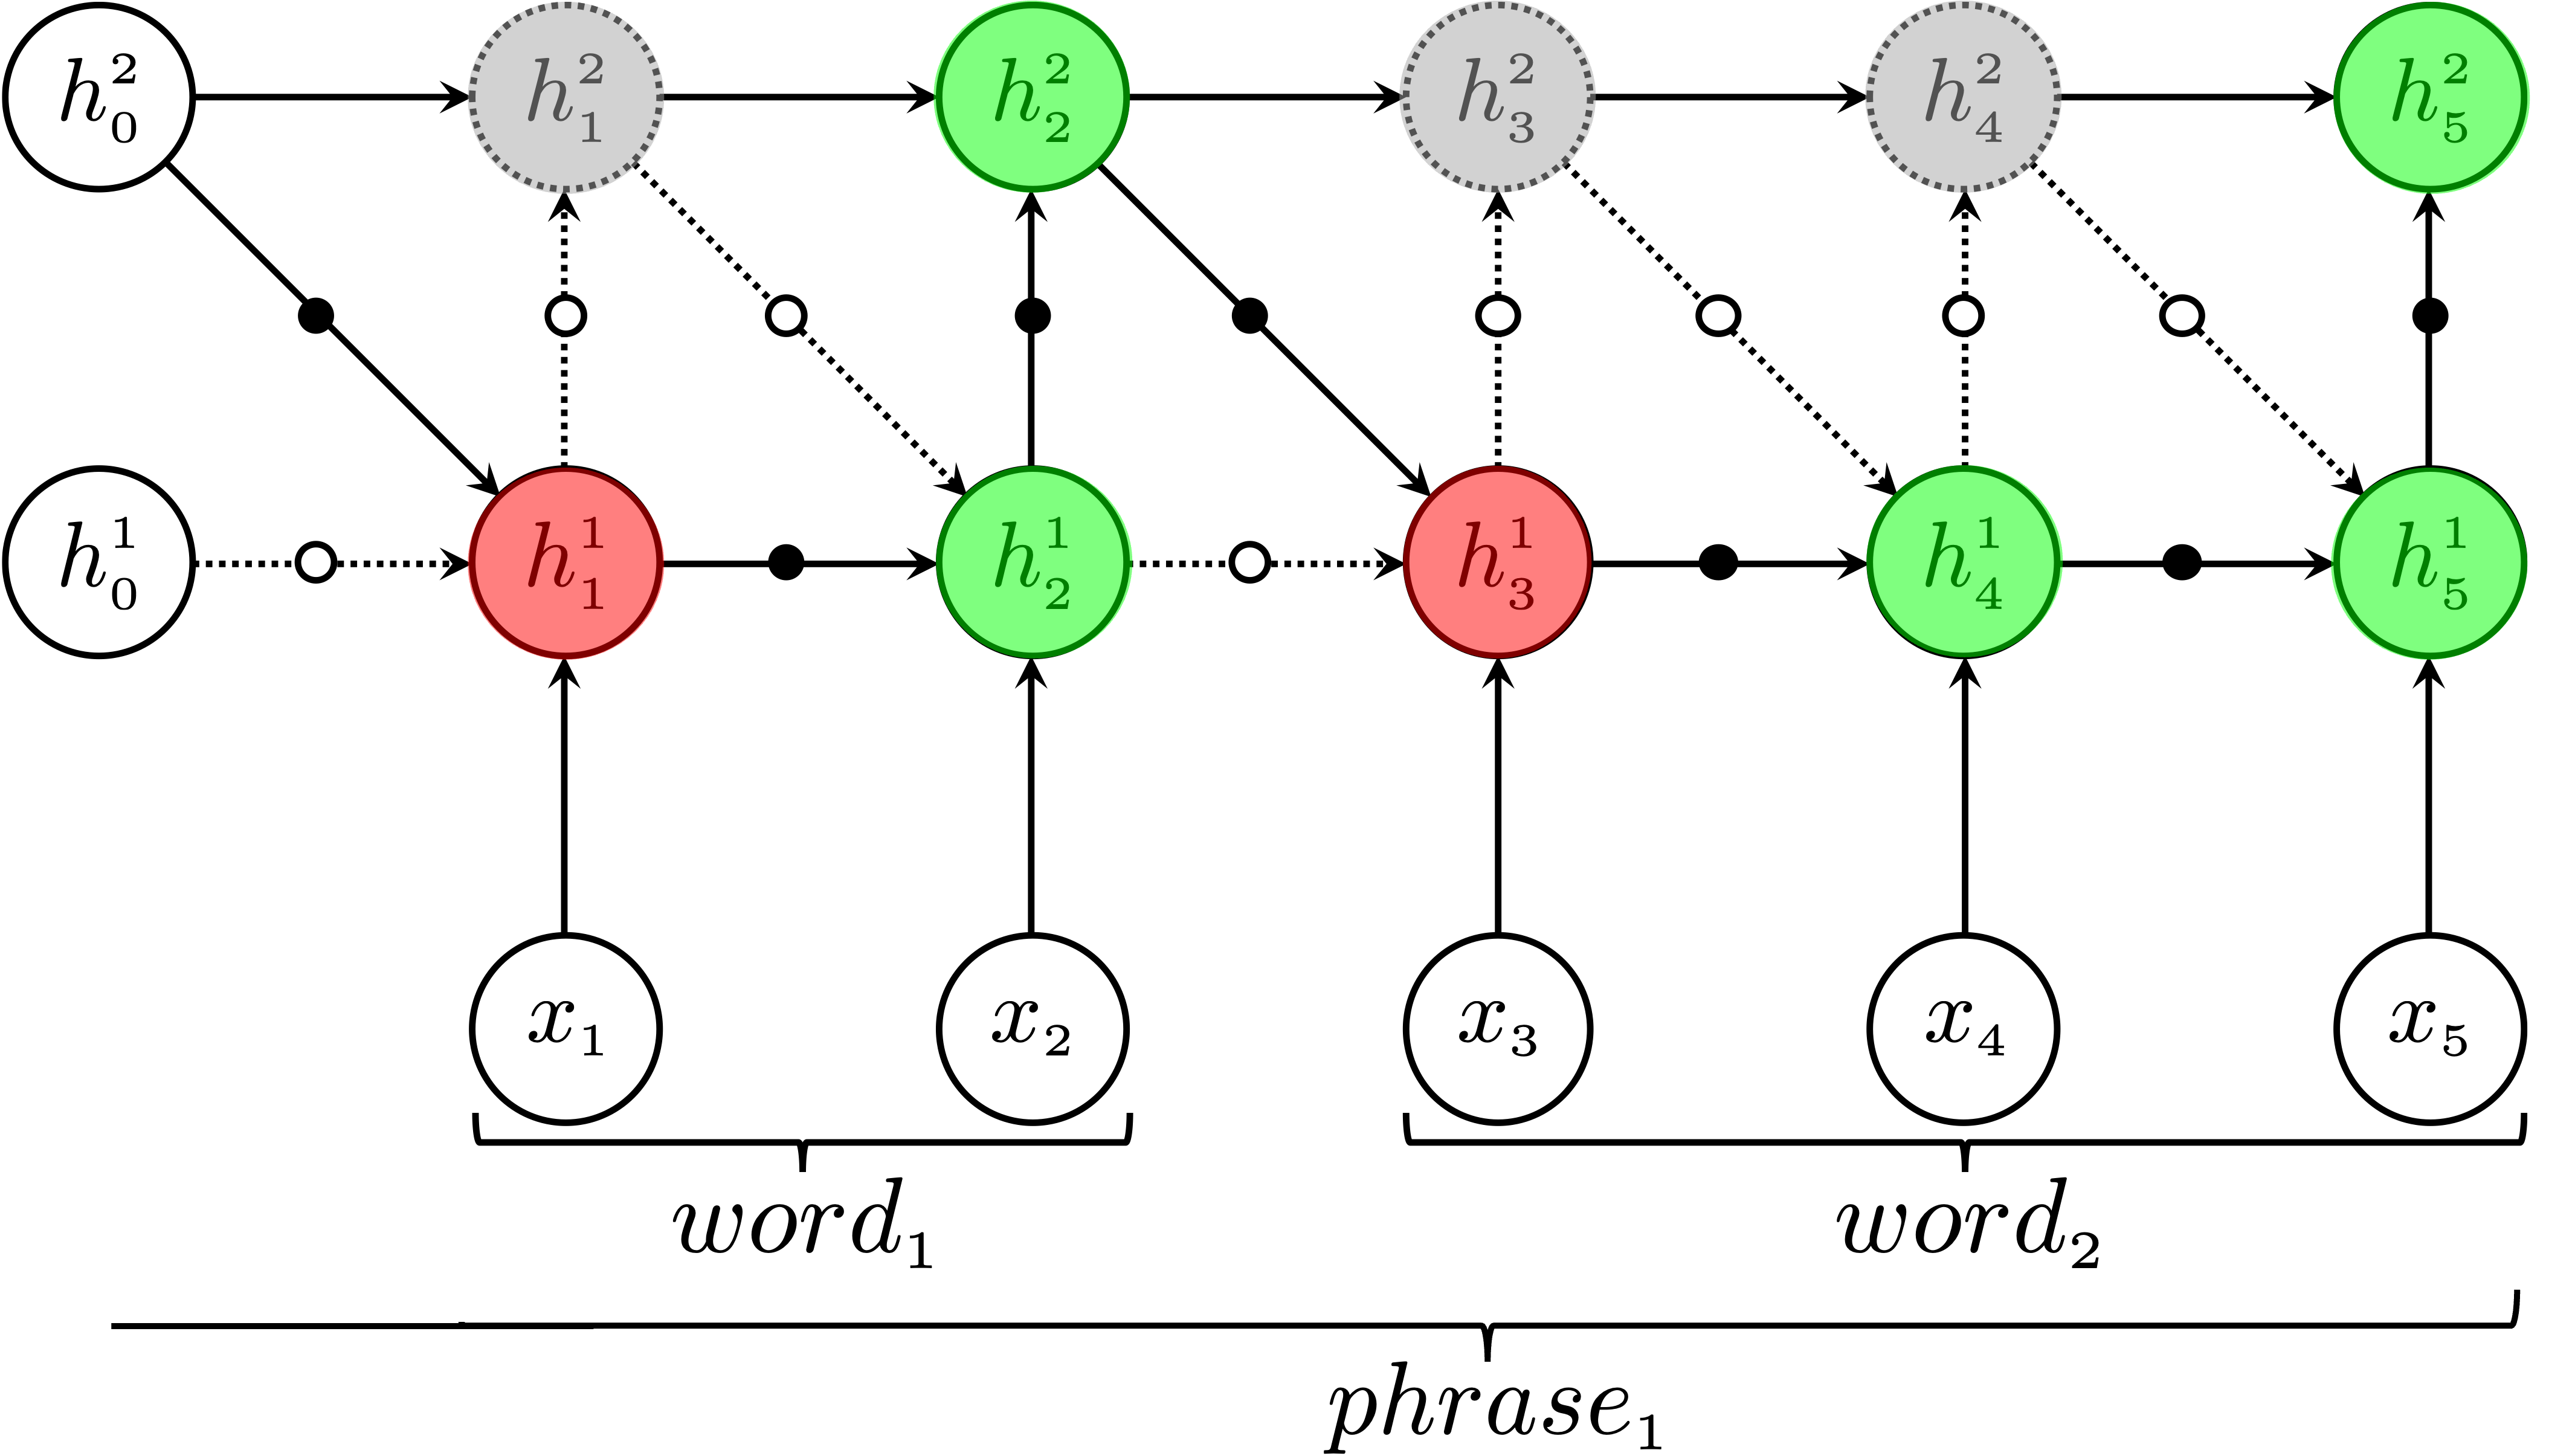
\includegraphics[scale=0.21]{architecture-ops.png}
\caption{\scriptsize{The HM-RNN architecture that discovers the hierarchical multiscale structure in the data without explicit boundary information. Units are color-coded based on the operation performed at each corresponding time step: green, gray or red for an UPDATE, a COPY or a FLUSH operation respectively.
}}

\label{fig:intuition}
\end{figure}
\end{columns}
\vspace{8pt}
\begin{myblock}{Update Mechanism}
At each time step, based on the state of boundary detectors, one of the following operations is executed:
\begin{itemize}
\item \greenhighlight{\textbf{UPDATE}}: similar to the update rule of LSTMs only that it is executed sparsely according to the boundary detectors (performed if the layer below detected a boundary at the current time step and no boundary was detected by the layer at the previous time step)
\item \grayhighlight{\textbf{COPY}}: simply a copy of the cell and hidden states of the previous time step (executed when no boundaries are detected)
\item \redhighlight{\textbf{FLUSH}}: involves ejecting the summarized representation of the current segment to the upper layer and erasing the state to start processing the next segment (executed if the layer detected a boundary at the previous time step)
\end{itemize}
\end{myblock}
\end{frame}
%%%%%%%%%%%%%%%%%%%%%%%%%%%%%%%%%%%%%%%%%%%%%%%%%%%%%%%%%
\begin{frame}[shrink=53]{Model description -- Details}
\footnotesize
\begin{columns}[t]
\column[T]{.7\textwidth}
\begin{myblock}{Hierarchical Multiscale LSTM (HM-LSTM)}
In a HM-LSTM model of $L$ layers ($\ell = 1, \ldots, L$), at time step $t$, each layer $\ell$ performs the following update
$$\mathbf{h}_t^\ell,\mathbf{c}_t^\ell,z_t^\ell = f_{\text{HM-LSTM}}^\ell (\mathbf{c}_{t-1}^\ell ,\mathbf{h}_{t-1}^\ell ,\mathbf{h}_{t}^{\ell-1},\mathbf{h}_{t-1}^{\ell+1},z_{t-1}^\ell ,z_t^{\ell-1})$$
$$
\mathbf{c}_t^\ell=
\begin{cases}
\mathbf{f}_t^\ell\odot \mathbf{c}_{t-1}^\ell + \mathbf{i}_t^\ell \odot \mathbf{g}_t^\ell & \text{if }z_{t-1}^\ell=0\text{ and }z_t^{\ell-1}=1\text{ (UPDATE)}\\
\mathbf{c}_{t-1}^\ell & \text{if }z_{t-1}^\ell=0\text{ and }z_t^{\ell-1}=0\text{ (COPY)}\\
\mathbf{i}_t^\ell\odot \mathbf{g}_t^\ell & \text{ if }z_{t-1}^\ell=1\text{ (FLUSH)}
\end{cases}
$$
$$\mathbf{h}_t^\ell=\begin{cases}\mathbf{h}_{t-1}^\ell & \text{ if COPY}\\ \mathbf{o}_t^\ell\odot \texttt{tanh}(\mathbf{c}_t^\ell)&\text{ otherwise}\end{cases}$$
where $\mathbf{h}$ ( $\mathbf{h}_t^0=\mathbf{x}_t$), $\mathbf{c}$ and $z$ denote the hidden, the cell and the boundary detector state, respectively, while $(\textbf{f}_t^\ell, \textbf{i}_t^\ell, \textbf{o}_t^\ell)$ are forget, input and output gates and $\textbf{g}_t^\ell$ denotes a cell proposal vector, whose values are given by
$$
\begin{pmatrix}
\mathbf{f}_t^\ell\\
\mathbf{i}_t^\ell\\
\mathbf{o}_t^\ell\\
\mathbf{g}_t^\ell\\
\tilde{z}_t^\ell\\
\end{pmatrix} =
\begin{pmatrix}
\texttt{sigm}\\
\texttt{sigm}\\
\texttt{sigm}\\
\texttt{tanh}\\
\texttt{hard-sigm}
\end{pmatrix}f_{\texttt{slice}}(\underset{\cyanhighlight{\mathbf{s}_t^{\text{\rmfamily{recurrent}}(\ell)}}}{\underbrace{(1-z_{t-1}^{\ell})U_{\ell}^{\ell}\mathbf{h}_{t-1}^\ell}} + \underset{\magentahighlight{\mathbf{s}_t^{\text{\rmfamily{top-down}}(\ell)}}}{\underbrace{z_{t-1}^{\ell}U_{\ell+1}^{\ell}\mathbf{h}_{t-1}^{\ell+1}}}+\underset{\yellowhighlight{\mathbf{s}_t^{\text{\rmfamily{bottom-up}}(\ell)}}}{\underbrace{z_{t}^{\ell-1}W_{\ell-1}^{\ell}\mathbf{h}_{t}^{\ell-1}
}}+\mathbf{b}^\ell)$$
$U_i^j\in \mathbb{R}^{(4dim(\mathbf{h}^j)+1)\times dim(\mathbf{h}^i)}$, $W_i^j\in \mathbb{R}^{(4dim(\mathbf{h}^j)+1)\times dim(\mathbf{h}^{i})}$ denote state transition parameters from layer $i$ to layer $j$, $\mathbf{b}^{\ell}\in \mathbb{R}^{4dim(\mathbf{h}^\ell)+1}$ is a bias term and \texttt{hard-sigm}$(x)=\max(0, \min(1,\frac{ax+1}{2}))$ with $a$ being a slope variable.

The binary boundary state $z_t^\ell$ could be obtained by
$$z_t^\ell=\begin{cases}1 & \text{ if }\tilde{z}_t^\ell>0.5\\ 
0 & \text{ otherwise}\end{cases}$$
or sampling from a Bernoulli distribution ($z_t^\ell \sim \text{Bernoulli}(\tilde{z}_t^\ell)$). Since the input should not be omitted, $z_t^0=1$ for all $t$.
\end{myblock}
\begin{myblock}{The Slope Annealing Trick}
\begin{itemize}
\item To backpropagate $z_t^\ell$, use the \textbf{Straight-Through Estimator} \cite{hinton2012neural}: replace the step function used in the forward pass (non-differentiable) with the \texttt{hard-sigmoid} (differentiable).
\item To reduce the discrepancy between the two functions used during the forward pass and the backward pass, gradually increase the slope $a$ of the \texttt{hard-sigmoid} function.
\end{itemize}
\end{myblock}
\column[T]{.28\textwidth}
\begin{myblock}{Standard LSTM}
For comparison, in a LSTM model with a single layer, at time step $t$, the following operations are performed
$$\mathbf{h}_t, \mathbf{c}_t=f_{LSTM}(\mathbf{c}_{t-1}, \mathbf{h}_{t-1})$$
$$\mathbf{c}_t=\mathbf{f}_t\odot \mathbf{c}_{t-1}+\mathbf{i}_t\odot \mathbf{g}_t$$
$$\mathbf{h}_t=\mathbf{o}_t\odot \texttt{tanh}(\mathbf{c}_t)$$
$$
\scriptsize{
\begin{pmatrix}
\mathbf{f}_t\\
\mathbf{i}_t\\
\mathbf{o}_t\\
\mathbf{g}_t\\
\end{pmatrix} =
\begin{pmatrix}
\texttt{sigm}\\
\texttt{sigm}\\
\texttt{sigm}\\
\texttt{tanh}\\
\end{pmatrix}f_{\texttt{slice}}(
U\mathbf{h}_{t-1}+W\mathbf{x}_{t}+\mathbf{b})}
$$
%where $U\in\mathbb{R}^{4dim(\mathbf{h})\times dim(\mathbf{h})}$, $W\in\mathbb{R}^{4dim(\mathbf{x})\times dim(\mathbf{x})}$, $\mathbf{b}\in\mathbb{R}^{4dim(\mathbf{h})}$.
\end{myblock}
\vspace{-6pt}
\begin{figure}
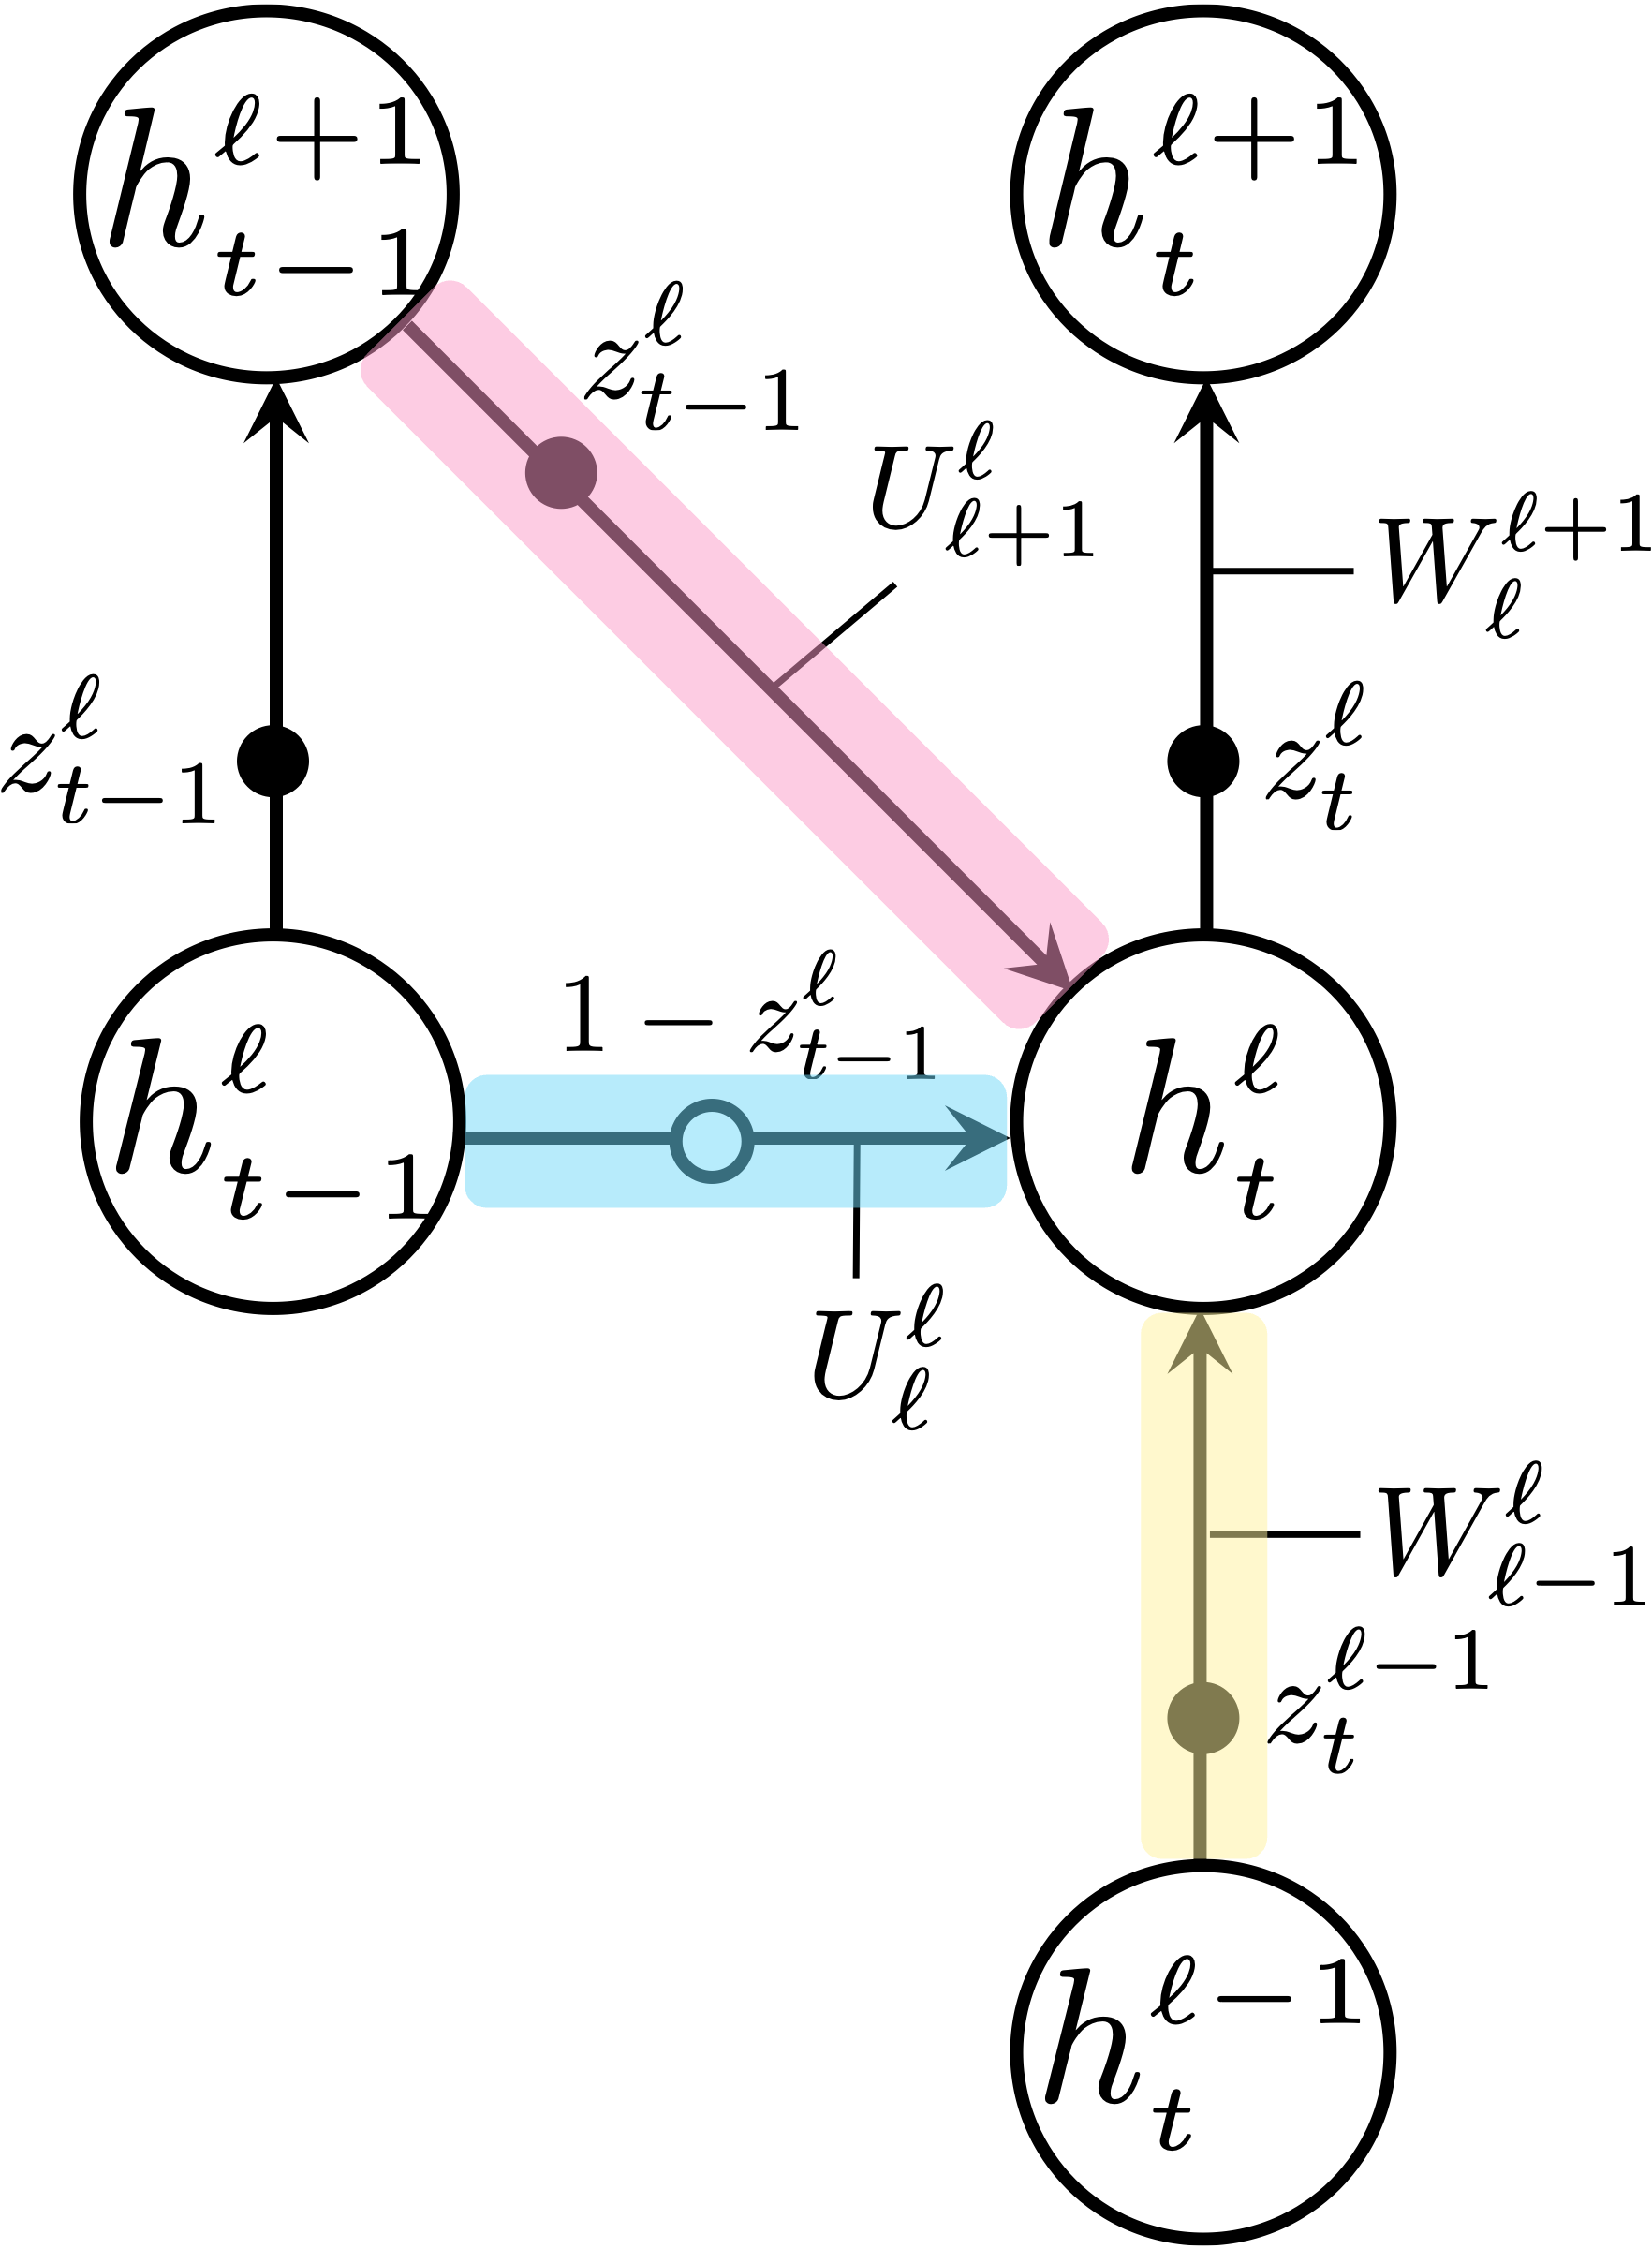
\includegraphics[scale=0.47]{architecture-weights.png}
\caption{Gating mechanism of the HM-LSTM.}
\label{fig:architecture}
\end{figure}
\end{columns}
\vspace{12pt}
\hrule
\vspace{2pt}
\scriptsize{In the paper $\mathbf{s}_t^{\text{\rmfamily{recurrent}}(\ell)}$ does not include the factor $(1-z_{t-1}^{\ell})$, however this contrasts with the definition of the FLUSH operation (that should perform a 'hard' reset) and with the diagram in Figure \ref{fig:architecture}. Furthermore, the dimensions of $W_i^j$ and $U_i^j$ were wrongly defined.}
\end{frame}
%%%%%%%%%%%%%%%%%%%%%%%%%%%%%%%%%%%%%%%%%%%%%%%%%%%%%%%%%
\begin{frame}[shrink=20]{Model description -- Key points}
\footnotesize \let\small\footnotesize % makes subitems smaller too
\begin{myblock}{Key Features of the Model}
\begin{itemize}
\item The model \textbf{discovers} underlying hierarchical structure in sequences \textbf{without using explicit boundary information}
\item Unlike the LSTM, $\mathbf{f}, \mathbf{i}, \mathbf{o}$ and $\mathbf{g}$ do not need to be computed at every time step, \textbf{reducing computational costs} (e.g., in case of COPY none of them needs to be computed)
\item The top down connection from layer $(\ell+1)$ to $(\ell)$ makes the layer $(\ell)$ to be \textbf{initialized} with more \textbf{long-term information} (i.e., a broader context) after a boundary is detected
\item The model employs the \textbf{multiscale update} concept:
\begin{itemize}
\item an UPDATE at a layer can occur only after at least one UPDATE is performed at its previous layer, resulting in a lower frequency of updates at higher layers compared to lower ones
\end{itemize}
\item The COPY operation retains the whole state without any loss of information, \textbf{improving gradient propagation} (similar to Zoneout \cite{krueger2016zoneout}, but instead of being randomly applied, is performed based on the input)
\item The FLUSH operation \textbf{passes a summary information} to the upper layer (allowing it to build its higher-level representation) and, differently from the forget operation in LSTM, it \textbf{completely erases the previous state} of the layer. Furthermore, it \textbf{incorporates both a reward} (feeding fresh information to upper layers) and a \textbf{penalty} (erasing accumulated information).
\item To compute the target, the model \textbf{considers representations at every level of abstraction}, not solely those at the higher levels (see Figure \ref{fig:output_layer})
\end{itemize}
\end{myblock}
\end{frame}
%%%%%%%%%%%%%%%%%%%%%%%%%%%%%%%%%%%%%%%%%%%%%%%%%%%%%%%%%
\begin{frame}[shrink=28]{Experiments}
\footnotesize
\begin{columns}[t]
\column[t]{.5\textwidth}
\begin{myblock}{Character-level Language Modeling}
\begin{itemize}
\item \textbf{Task}: predict the next character, i.e., discrete sequence modeling
\item \textbf{Datasets}: Penn Treebank \cite{marcus1993building}, Text8 \cite{mahoney2011large}, Hutter Prize Wikipedia \cite{hutter2012human}
\item \textbf{Evaluation metric}: Bits-per-character, $BPC=\mathbb{E}[-\log_2p(x_{t+1}|x_{\leq t})]$ 
\end{itemize}
\end{myblock}
\column[t]{.48\textwidth}
\begin{myblock}{Handwriting Sequence Generation}
\begin{itemize}
\item \textbf{Task}: predict the next pen coordinates and pen state (up or down), i.e., real-valued sequence modeling
\item \textbf{Dataset}: IAM-OnDB \cite{liwicki2005iam}
\item \textbf{Evaluation metric}: Average Log-Likelihood
\end{itemize}
\vspace{6pt}
\end{myblock}
\end{columns}
\vspace{5pt}
\begin{columns}[t]
\column[t]{.65\textwidth}
\begin{myblock}{Model Architecture}
\begin{itemize}
\item \textbf{Input Embedding Layer}: maps each input symbol into a 128-dimensional continuous vector without using any non-linearity 
\item \bluehighlight{\textbf{3 HM-LSTM Layers}} (512 units on Penn Treebank, 1024 units on Text8 and Hutter Prize Wikipedia, 400 units on IAM-OnD)
\item \violethighlight{\textbf{Output Embedding Layer}}: a feedforward neural network (512 units  on Penn Treebank, 2048 units on Text8 and Hutter Prize Wikipedia, 400 units on IAM-OnD) receiving at each time step the hidden states of the three HM-LSTM layers, adaptively weighted by additional scalar gating units (Figure \ref{fig:output_layer})
\item \orangehighlight{\textbf{Output Layer}}: softmax layer for character-level language modeling, Mixture Density Network \cite{graves2013generating} for handwriting sequence generation
\end{itemize}
\end{myblock}
\column[t]{.30\textwidth}
\vspace{20pt}
\begin{figure}
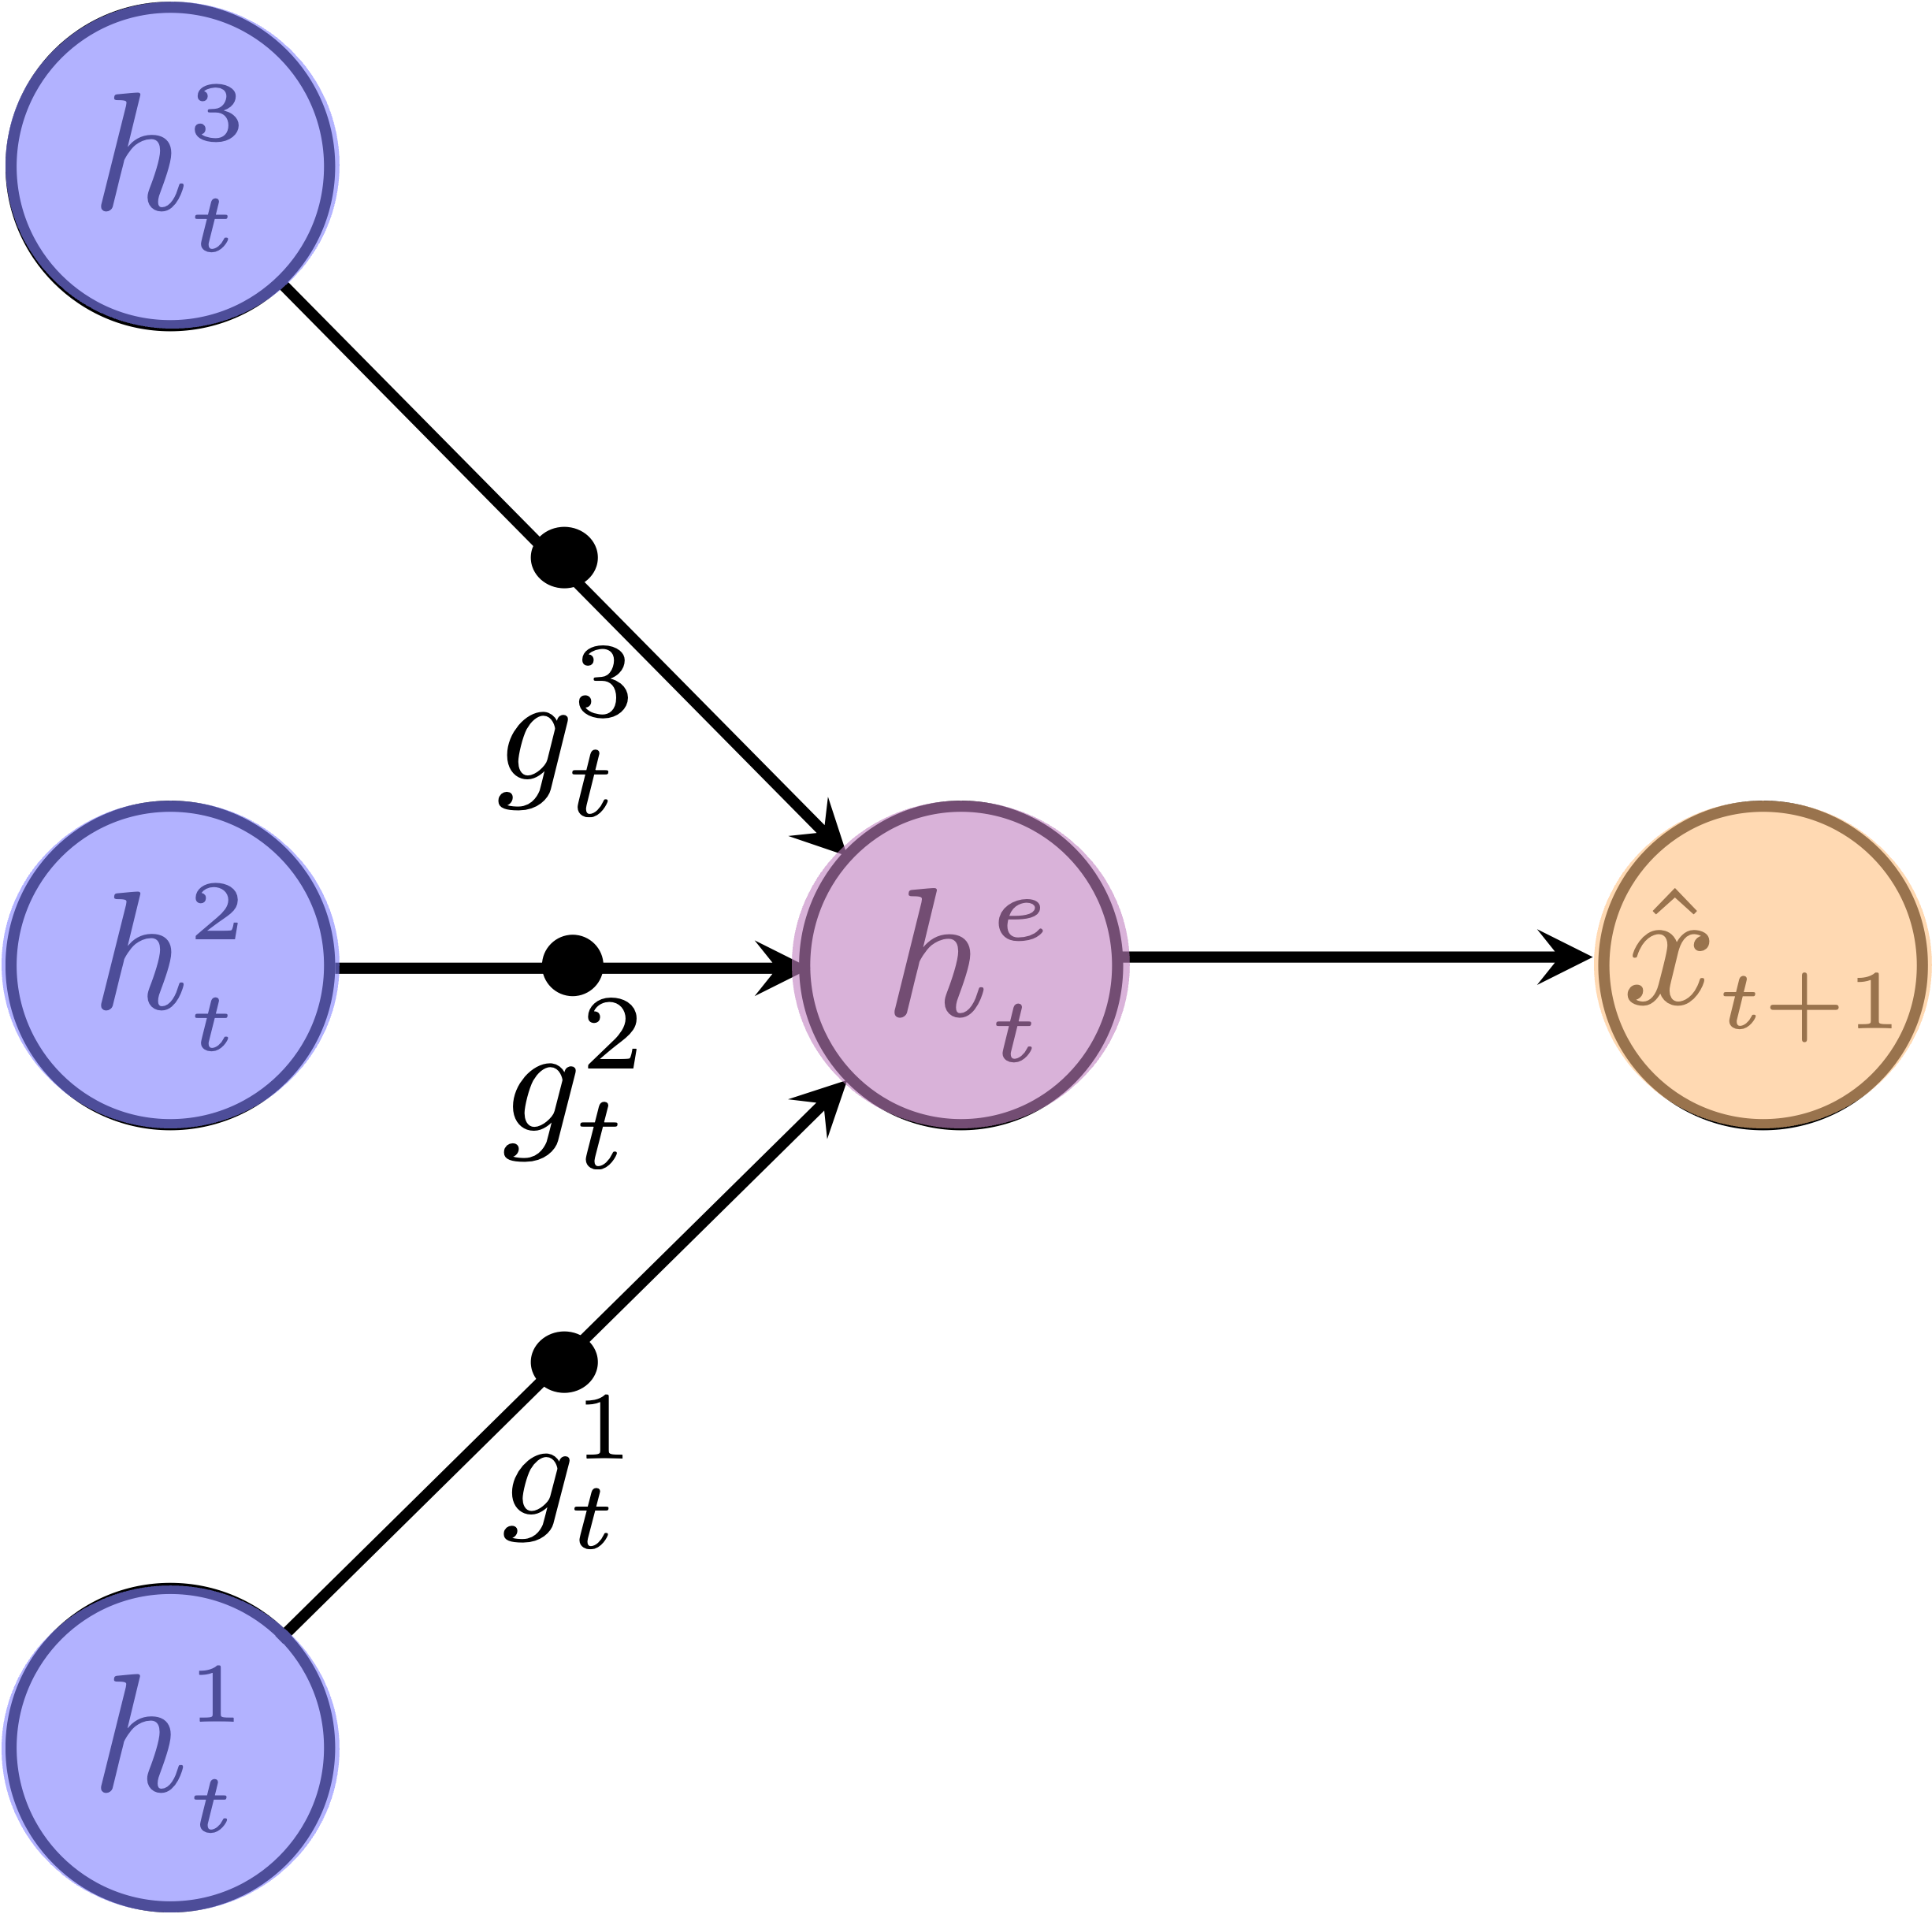
\includegraphics[scale=0.22]{output-module.png}
\caption{Output Embedding Layer.}
\label{fig:output_layer}
\end{figure}
\end{columns}
\end{frame}
%%%%%%%%%%%%%%%%%%%%%%%%%%%%%%%%%%%%%%%%%%%%%%%%%%%%%%%%%
\begin{frame}[shrink=40]{Results}
\centering
\vspace{-25pt}
\footnotesize{
\begin{table}
\caption{Results for character-level language modeling.}
\begin{tabular}
{lr|lr|lr}
\toprule
\multicolumn{2}{c|}{\textbf{Penn Treebank}} & \multicolumn{2}{c|}{\textbf{Text8}} & \multicolumn{2}{c}{\textbf{Hutter Prize Wikipedia}}\\
\midrule
\textbf{Model} & \textbf{BPC} & \textbf{Model} & \textbf{BPC} & \textbf{Model} & \textbf{BPC}\\
LayerNormHyperNetworks \cite{ha2016hypernetworks} & \textbf{1.23} &  BatchNorm LSTM \cite{cooijmans2016recurrent} & 1.36 & Recurrent Highway Networks \cite{zilly2017recurrent} & 1.32\\
{\usebeamercolor[fg]{structure}LayerNorm HM-LSTM Sampling} & 1.27 & {\usebeamercolor[fg]{structure}HM-LSTM} & 1.32 & decomp8 \cite{mahoney2011large} ** & \textbf{1.28}\\
{\usebeamercolor[fg]{structure}LayerNorm HM-LSTM Soft *} & 1.27 & {\usebeamercolor[fg]{structure}LayerNorm HM-LSTM} & \textbf{1.29} & {\usebeamercolor[fg]{structure}HM-LSTM} & 1.34\\
{\usebeamercolor[fg]{structure}LayerNorm HM-LSTM Step} & 1.25 & & & {\usebeamercolor[fg]{structure}LayerNorm HM-LSTM} & 1.32\\
{\usebeamercolor[fg]{structure}LayerNorm HM-LSTM Step \& SA} & 1.24 & &\\
\bottomrule
\end{tabular}\\
\scriptsize{* a variant of HM-LSTM that does not discretize the boundary detector states; ** compression-based model (non-neural)}
\end{table}
}
\vspace{-25pt}
\begin{columns}
\column[t]{.5\textwidth}
\vspace{4pt}
\begin{myblock}{Findings}
\begin{itemize}
\normalsize{
\item \textbf{PennTreebank}: comparable results to SotA; best score achieved with the Slope Annealing (SA) trick
\item \textbf{Text8}: SotA results
\item \textbf{Hutter Prize Wikipedia}: tie with SotA results among neural models
\item \textbf{IAM-OnDB}: better than standard LSTM; best score achieved with the SA trick
\item The \textbf{discovered hierarchical structure is very similar to the intrinsic structure} observed in the data: $z^1$ tends to be turned on when it sees a space or after it sees a space;  $z^2$ tends to fire when it sees either the end of a word or 2, 3-grams (Figure \ref{fig:discovered_hierarchy})
}
\end{itemize}
\vspace{10pt}
\end{myblock}
\column[t]{.48\textwidth}
\vspace{-20pt}
\footnotesize{
\begin{table}
\caption{Results for handwriting sequence generation.}
\begin{tabular}
{lr}
\toprule
\multicolumn{2}{c}{\textbf{IAM-OnDB}}\\
\midrule
\textbf{Model} & \textbf{Average Log-Likelihood}\\
Standard LSTM \cite{hochreiter1997long} & 1081\\
{\usebeamercolor[fg]{structure}HM-LSTM} & 1137\\
{\usebeamercolor[fg]{structure}HM-LSTM Step \& SA} & \textbf{1167}\\
\bottomrule
\end{tabular}
\end{table}
}
\begin{figure}
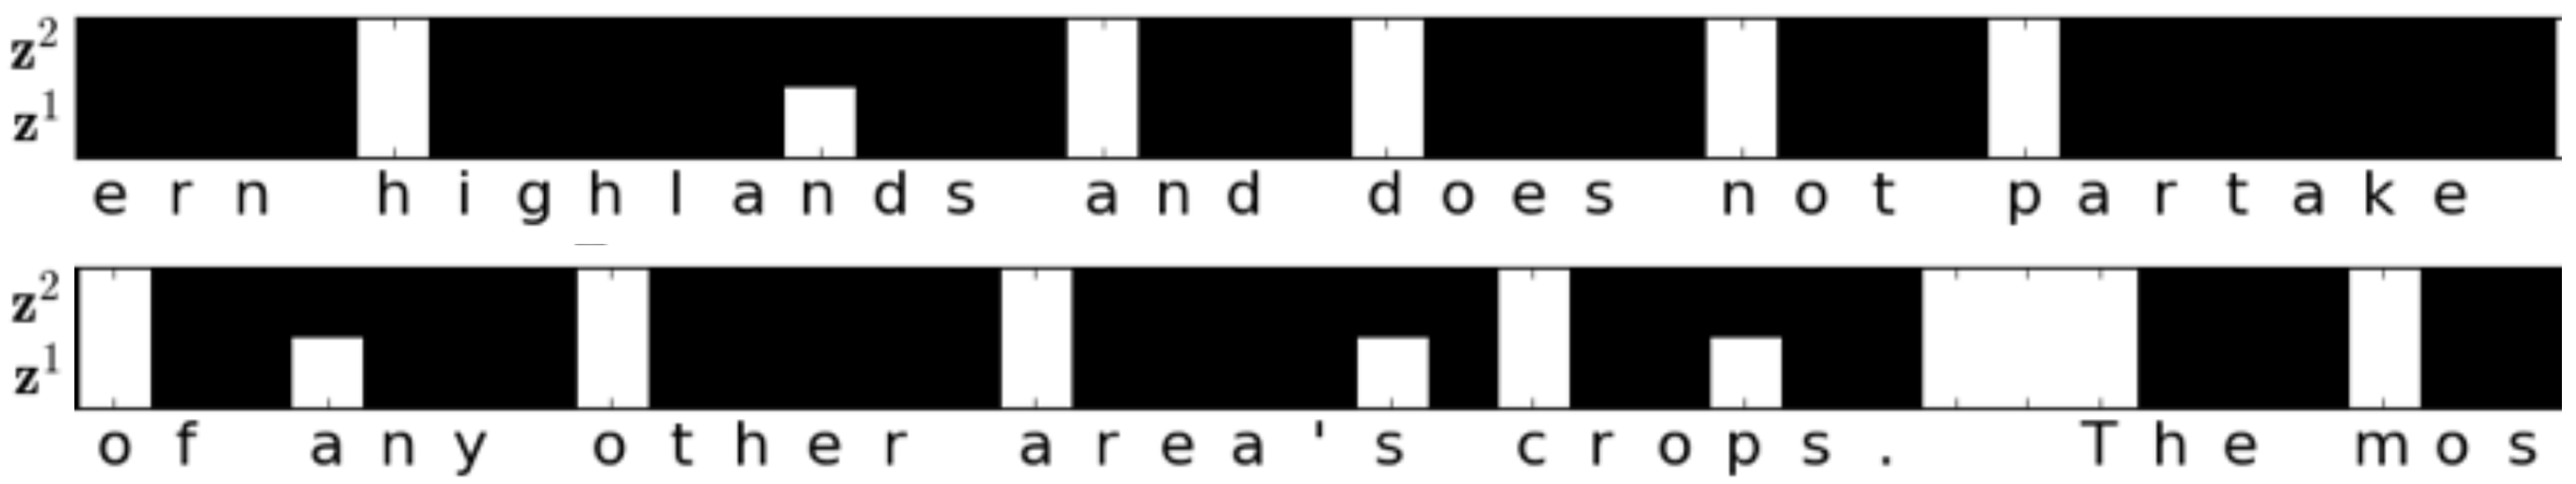
\includegraphics[scale=0.18]{boundaries.png}
\caption{Discovered hierarchical multiscale structure in the first line of the Hutter Prize Wikipedia dataset ($z^l=1$ in white, $z^l=0$ in black).}
\label{fig:discovered_hierarchy}
\end{figure}
\end{columns}
\end{frame}
%%%%%%%%%%%%%%%%%%%%%%%%%%%%%%%%%%%%%%%%%%%%%%%%%%%%%%%%%
\begin{frame}[shrink=24]{Comments}
\footnotesize \let\small\footnotesize % makes subtimes smaller too
\begin{exampleblock}{Pros}
\begin{itemize}
\item \textbf{Novelties}:
\begin{itemize}
\item The model \textbf{learns latent hierarchical structure} of sequences without using explicit boundary information
\item The \textbf{Slope Annealing Trick}, proven effective and potentially applicable in other contexts
\end{itemize}
\item \textbf{Computational efficiency}: upper layers are updated less frequently
\item Efficacy in capturing \textbf{long term dependencies}: less frequent updates reduce the gradient vanishing problem
\item Flexible \textbf{resource allocation}: may allocate more units to higher layers, which model long-term dependencies, without significantly increasing computational costs
\item \textbf{Interpretability}: discrete variables allow to inspect the discovered hierarchical structure
\item \textbf{State-of-the-art results} (or comparable performance) on several datasets
\end{itemize}
\end{exampleblock}
\begin{alertblock}{Cons}
\begin{itemize}
\item The use of discrete variables ($z$ variables) makes the model \textbf{no longer differentiable} and the Slope Annealing Trick requires finding a good schedule, which may not be feasible with large-scale datasets
\item Results on the claimed computational savings were not provided because, at the time of publication, it was \textbf{not entirely clear how to implement the state conditional computation in a mini-batch setting} \cite{review}
\item \textbf{Experiments were limited} to two tasks, and hierarchies beyond three levels were not investigated
\item Current SotA results in the studied tasks are achieved by transfomer-based models \cite{radford2019language}
\end{itemize}
\end{alertblock}
\end{frame}
%%%%%%%%%%%%%%%%%%%%%%%%%%%%%%%%%%%%%%%%%%%%%%%%%%%%%%%%
\begin{frame}[shrink=50]{References}
\begin{multicols}{2}
\footnotesize
\nocite{chung2016hierarchical}
\printbibliography
\end{multicols}
\end{frame}
%%%%%%%%%%%%%%%%%%%%%%%%%%%%%%%%%%%%%%%%%%%%%%%%%%%%%%%%
\end{document}